% !TeX spellcheck = cs_CZ
%{\tikzset{external/prefix={tikz/FYZII/}}
% \tikzset{external/figure name/.add={ch31_}{}}
%---------------------------------------------------------------------------------------------------
% file fey2ch31.tex
%---------------------------------------------------------------------------------------------------
%=========================== Kapitola Tenzory ======================================================
\setchaptertoc
\chapter{Tenzory}\label{fyz:IIchapXXXI}

  \section{Tenzory polarizovatelnosti}\label{fyz:IIchapXXXIsecI}
    Fyzici mají ve zvyku zvolit nejednodušší příklad nějakého jevu a nazvat jej „fyzikou", přičemž
    komplikovanější příklady nechávají na starosti jiným odvětvím, například aplikované matematice,
    elektroinženýrství, chemii nebo krystalografii. Dokonce i fyzika pevných látek je téměř
    „polofyzikou”, neboť se příliš zajímá o speciální látky. Proto i v těchto přednáškách budeme
    vynechávat spoustu zajímavých věcí. Například jednou z důležitých vlastností krystalů, nebo
    většiny látek, je to, že jejich elektrická polarizovatelnost je v různých směrech různá.
    Nachází-li se látka ve elektrickém poli, které má určitý směr, posunou se mírně náboje atomů a
    vytvoří se dipólový moment. Velikost tohoto momentu silně závisí na směru pole. A to je,
    samozřejmě, určitá komplikace. Ale ve fyzice si to zjednodušujeme a obvykle začínáme se
    speciálním případem, kdy je polarizovatelnost stejná ve všech směrech. Ostatní případy necháváme
    na starosti jiným vědním oborům. Proto v našich dalších úvahách vůbec nebudeme potřebovat to, o
    čem budeme mluvit v této kapitole.
    
    Matematika tenzorů je zvláště užitečná při popisu těch vlastností látek, které závisejí na
    směru, ačkoliv je to jen jeden z příkladů jejího využití. Jelikož většina z vás se nemíní stát
    fyziky, ale budete se zabývat reálným světem, kde věci silně závisejí na směru, budete muset
    dříve či později používat tenzory. Abychom nic nevynechávali, pohovoříme o tenzorech. Chceme,
    aby naše chápání fyziky bylo co nejúplnější. Například náš výklad elektrodynamiky je úplný - tak
    úplný jako libovolný kurz elektřiny a magnetizmu, dokonce i pro fyzikální specializace na vysoké
    škole. Mechanika nebyla úplně ukončena, protože, když jsme ji probírali, nebyly ještě naše
    matematické znalosti na takové úrovni, abychom mohli hovořit o tématech, jako je princip
    nejmenšího účinku, lagranžiány, hamiltoniány atd., které představují elegantnější způsob popisu
    mechaniky. Ale s výjimkou obecné teorie relativity jsme všechny zákony mechaniky probrali. Naše
    elektřina a magnetizmus jsou kompletní a mnoho dalších oblastí je v podstatě uzavřeno. Kvantová
    mechanika přirozeně ne; musíme si něco nechat do budoucna. Ale co je tenzor, musíme vědět už
    nyní. 

    V kapitole \ref{fyz:IIchapXXX} jsme zdůrazňovali, že vlastnosti krystalických látek jsou v
    různých směrech různé, říkáme, že jsou anizotropní. Závislost indukovaného dipólového momentu na
    směru vnějšího elektrického pole je jen jedním z možných příkladů, ale právě ten si vybereme
    jako příklad tenzoru. Předpokládejme, že při daném směru elektrického pole je indukovaný
    dipólový moment objemové jednotky \(\vec{P}\) úměrný intenzitě vnějšího pole \(\vec{E}\). (To je
    dobrá aproximace pro většinu látek, pokud \(\vec{E}\) není příliš velké.) Konstantu úměrnosti
    označíme \(\alpha\)\footnote{V kapitole \ref{fyz:IIchapX} jsme souhlasně s konvencí psali
    \(P=\varepsilon_0\chi E\) a \(\chi\) („chí") jsme nazývali \emph{susceptibilita}. Nyni bude
    pohodlnější používat jedno písmeno, proto namísto \(\varepsilon_0\chi\) budeme psát \(\alpha\).
    Pro izotropní dielektrika platí \(\alpha = (\varepsilon_r - 1)\varepsilon_0\), kde
    \(\varepsilon_r\) je relativní permitivita (článek \ref{fyz:IIchapXsecIV})}. Budeme uvažovat
    látky, v nichž \(\alpha\) závisí na směru pole, jako například v krystalech podobných vápenci,
    který má tu vlastnost, že při průhledu vidíme obraz dvojitě. 

    Předpokládejme, že jsme zjistili, že v určitém krystalu vyvolává elektrické pole \(\vec{E}_1\),
    působící ve směru osy \(x\), polarizaci \(\vec{P}_1\) ve směru \(x\). Dále nechť elektrické pole
    \(\vec{E}_2\) ve směru osy \(y\), které má stejnou intenzitu jako \(\vec{E}_1\), vyvolává jinou
    polarizaci \(\vec{P}_2\) ve směru \(y\). Co by se stalo, kdyby elektrické pole působilo pod
    úhlem \ang{45}? Takové pole je superpozicí dvou polí působících podél os \(x\) a \(y\), proto
    polarizace \(\vec{P}\) bude vektorovým součtem \(\vec{P}_1\) a \(\vec{P}_2\), jak je znázorněno
    na obr. \ref{fyz:fig0874a}. Polarizace už nemá tentýž směr jako elektrické pole. Lze pochopit,
    proč tomu tak je. V látce se mohou nacházet náboje, které se mohou snadno posouvat směrem nahoru
    a dolů, ale obtížně se pohybují ze strany na stranu. Když síla působí pod úhlem \ang{45}, náboje
    se posunou víc směrem nahoru než na stranu. Výsledné přemístění nemá směr vnější síly, protože
    tu působí vnitřní elastické síly, které jsou asymetrické.
    
    Úhel \ang{45} není, samozřejmě, nijak výjimečný. Indukovaná polarizace obecně nemá směr
    elektrického pole. V našem předcházejícím příkladě se nám „poštěstilo“ zvolit osy \(x\) a \(y\)
    tak, aby \(\vec{P}\) mělo směr \(\vec{E}\) podél obou os. Kdyby byl krystal pootočen vzhledem k
    osám souřadnic, vyvolalo by elektrické pole \(\vec{E}\) ve směru osy \(y\) polarizaci
    \(\vec{P}\), která by měla obě složky, \(x\) i \(y\). Podobně polarizace, která by vznikla díky
    poli ve směru osy \(x\), by také měla složky \(x\) i \(y\). Polarizace by potom vypadaly tak,
    jak je to na obr. \ref{fyz:fig0874b}, a ne jako na obr. \ref{fyz:fig0874a}. Věci se komplikují,
    ale stále je pro libovolné pole \(\vec{E}\) velikost \(\vec{P}\) \emph{úměrná} velikosti
    \(\vec{E}\). 
    
    Nyní uvažujme obecný případ libovolné orientace krystalu vzhledem k souřadnicovým osám.
    Elektrické pole ve směru osy \(x\) vede k polarizaci \(\vec{P}\) se složkami \(x\), \(y\), a
    \(z\). Můžeme psát
    \begin{equation}\label{fyz:eq236}
      P_x = \alpha_{xx}E_x, \quad P_y = \alpha_{yx}E_x, \quad  P_z = \alpha_{zx}E_x.
    \end{equation}

    Celé naše tvrzení je založeno na tom, že má-li elektrické pole směr osy \(x\), nemusí mít
    polarizace tentýž směr, ale má složky ve směru os \(x\), \(y\), \(z\) a každá z nich je úměrná
    \(E_x\). Konstanty úměrnosti označujeme \(\alpha_{xx}\), \(\alpha_{yx}\), \(\alpha_{zx}\).
    (První index je vztažen k příslušné složce \(\vec{P}\), druhý ke směru elektrického pole.) 
    
    Podobně pro pole ve směru osy \(y\) můžeme psát
    \begin{equation}\label{fyz:eq237}
      P_x = \alpha_{xy}E_y, \quad P_y = \alpha_{yy}E_y, \quad  P_z = \alpha_{zy}E_y.
    \end{equation}

    a pro pole ve směru osy \(z\)
    \begin{equation}\label{fyz:eq238}
      P_x = \alpha_{xz}E_z, \quad P_y = \alpha_{yz}E_z, \quad  P_z = \alpha_{zz}E_z.
    \end{equation}

    \begin{figure}[ht!]   %\ref{fyz:fig0874}
      \centering
      \subcaptionbox{\label{fyz:fig0874a}}{\luafigure[0.45]{fyz_fig0874a.pdf}}
      \subcaptionbox{\label{fyz:fig0874b}}{\luafigure[0.45]{fyz_fig0874b.pdf}}
      \caption{Vektorový součet polarizací v anizotropním krystalu (\cite[s.~748]{Feynman02})}
      \label{fyz:fig0874}
    \end{figure}

    Řekli jsme, že polarizace závisí na polích lineárně, proto má-li elektrické pole \(\vec{E}\)
    složku \(x\) i \(y\), bude výsledná \(x\)-ová složka \(\vec{P}\) součtem dvou \(P_x\) z rovnic
    (\ref{fyz:eq236}) a (\ref{fyz:eq237}). Má-li \(\vec{E}\) složky \(x\), \(y\) a \(z\) budou
    výsledné složky \(\vec{P}\) součtem tří příspěvků z rovnic (\ref{fyz:eq236}),
    (\ref{fyz:eq237}), (\ref{fyz:eq238}). Jinými slovy \(\vec{P}\) bude určeno rovnicemi
    \begin{align}\label{fyz:eq240}
      P_x &= \alpha_{xx}E_x + \alpha_{xy}E_y + \alpha_{xz}E_z  \nonumber \\
      P_y &= \alpha_{yx}E_x + \alpha_{yy}E_y + \alpha_{yz}E_z            \\
      P_z &= \alpha_{zx}E_x + \alpha_{zy}E_y + \alpha_{zz}E_z. \nonumber
    \end{align}

    Dielektrické vlastnosti krystalu jsou pak zcela určeny devíti veličinami (\(\alpha_{xx}\),
    \(\alpha_{xy}\), \(\alpha_{xz}\), \(\alpha_{yz}\) \(\ldots\)), které mohou být reprezentovány
    symbolem \(\alpha_{ij}\). (Indexy \(i\), \(j\) zastupují libovolné ze tří písmen \(x\), \(y\),
    \(z\)). Libovolné elektrické pole \(\vec{E}\) může být rozloženo na složky \(E_x\), \(E_y\),
    \(E_z\). Z nich můžeme použitím \(\alpha_{ij}\) najít \(P_x\), \(P_y\) a \(P_z\), které nám
    spolu určují polarizaci \(\vec{P}\). Soubor devíti koeficientů \(\alpha_{ij}\) se nazývá
    \textbf{tenzor} - v tomto případě \textbf{tenzor polarizovatelnosti}. Když říkáme, že tři čísla
    (\(E_x\), \(E_y\), \(E_z\)) tvoří vektor \(\vec{E}\), stejně říkáme, že devět čísel
    (\(\alpha_{xx}\), \(\alpha_{xy}\), \(\alpha_{xz}\), \(\alpha_{yz}\) \(\ldots\)) tvoří tenzor
    \(\alpha_{ij}\). 

  \twocolumn[\section{Transformace tenzorových složek}\label{fyz:IIchapXXXIsecII}]
    Víme, že při přechodu k nové souřadnicové soustavě \(x'\), \(y'\), \(z'\) dostáváme jiné složky
    \(E_{x'}\), \(E_{y'}\),  \(E_{z'}\) vektoru \(\vec{E}\) a stejně i jiné \emph{složky} vektoru
    \(\vec{P}\). Proto všechny koeficienty \(\alpha_{ij}\) mají různou hodnotu v různých
    souřadnicových soustavách. Změnu koeficientů \(\alpha\) při změně \(\vec{E}\) a \(\vec{P}\) lze
    zjistit, neboť popisujeme-li \emph{stejné fyzikální} elektrické pole v nové souřadnicové
    soustavě, měli bychom dostat stejnou polarizaci. Pro libovolnou novou souřadnicovou soustavu je
    \(P_{x'}\) lineární kombinací \(P_{x}\), \(P_{y}\), a \(P_{z}\):
    \begin{equation*}
      P_{x'} = aP_x + bP_y + cP_z.
    \end{equation*}
    Podobně je to i pro ostatní složky. Dosadíme-li za \(P_{x}\), \(P_{y}\), a \(P_{z}\), jejich
    vyjádření pomocí \(\vec{E}\) rovnic (\ref{fyz:eq240}), dostaneme
    \begin{align*}
      P_{x'} = &a(\alpha_{xx}E_x + \alpha_{xy}E_y + \alpha_{xz}E_z) + \\
               &b(\alpha_{yx}E_x + \alpha_{yy}E_y + \alpha_{yz}E_z) + \\
               &c(\alpha_{zx}E_x + \alpha_{zy}E_y + \alpha_{zz}E_z).
    \end{align*}
    Pak vyjádříme \(E_{x}\), \(E_{y}\), a \(E_{z}\), pomocí \(E_{x'}\), \(E_{y'}\), a \(E_{z'}\),
    například
    \begin{equation*}
      E_x =  a'E_x + b'E_y + c'E_z,
    \end{equation*}
    kde \(a'\), \(b'\), \(c'\) jsou v nějakém vztahu k \(a\), \(b\), \(c\), ale navzájem si nejsou
    rovny. Vyjádřili jsme tedy \(P_{x'}\) pomocí složek \(E_{x'}\), \(E_{y'}\), a \(E_{z'}\), tj.
    máme nové \(\alpha_{ij}\). To je trochu neuspořádaný, ale přímočarý postup.

    Když mluvíme o změně os, předpokládáme, že poloha krystalu v prostoru je fixována. Kdyby se
    krystal otáčel \emph{společně} s osami, koeficienty \(\alpha\) by se neměnily. Naopak, kdyby se
    orientace krystalu vzhledem k osám změnila, dostali bychom nový soubor hodnot \(\alpha\).
    Známe-li však koeficienty \(\alpha\) pro nějakou libovolnou orientaci krystalu, můžeme je najít
    pro libovolnou jinou orientaci pomocí transformace, kterou jsme právě popsali. Jinými slovy,
    dielektrické vlastnosti jsou \emph{úplně} popsány zadáním složek polarizovatelnosti tenzoru
    \(\alpha_{ij}\) vzhledem k libovolně zvolené soustavě souřadnic. Stejně jako částici přiřazujeme
    vektor rychlosti \(\vec{v} = (v_x, v_y, v_z)\), vědomi si toho, že tři složky se určitým
    způsobem mění při změně souřadnicových os, podobně krystalu přiřazujeme tenzor
    polarizovatelnosti \(\alpha_{ij}\), jehož devět složek se při změně souřadnicové soustavy
    transformuje určitým způsobem.

    Vztah mezi \(\vec{P}\) a \(\vec{E}\) určený rovnicí (\ref{fyz:eq240}) můžeme zapsat ve zkráceném
    tvaru
    \begin{equation}\label{fyz:eq241}
      P_i = \sum_j\alpha_{ij}E_j,
    \end{equation}

    kde \(i\) označuje některé z písmen \(x\), \(y\) nebo \(z\) a sčítáme přes \(j = x, y, z\). Pro
    operace s tenzory bylo vynalezeno mnoho speciálních označení, ale každé z nich se hodí jen pro
    omezenou třídu problémů. Jednou z obecných konvencí je vynechávání sumačního znaku \(\sum\) v
    rovnici (\ref{fyz:eq241}), přičemž se rozumí, že všude, kde se stejný index vyskytuje dvakrát (v
    našem případě \(j\)), musíme sčítat přes všechny jeho hodnoty. Jelikož tenzory nebudeme používat
    často, nebudeme se trápit s výběrem speciálních označení a konvencí.

  \section{Elipsoid energie}\label{fyz:IIchapXXXIsecIII}
    Nyní si vyzkoušejme, jak se zachází s tenzory. Položíme si zajímavou otázku: Jaká energie je
    potřebná k polarizaci krystalu (kromě energie elektrického pole, o níž víme, že je rovna
    \(\varepsilon_0E^2/2\) pro objemovou jednotku)? Zamyslíme se nad atomovými náboji, které se
    posouvají. Práce, která je vykonána při přemisťování náboje o vzdálenost \(\dd{x}\), je
    \(qE_x\dd{x}\) a je-li v jednotkovém objemu \(N\) nábojů, je vykonaná práce  \(qE_xN\dd{x}\).
    Ale  \(qN\dd{x}\) je změna \(qP_x\), dipólového momentu objemové jednotky. Proto energie
    připadající na \emph{objemovou jednotku} je
    \begin{equation*}
      E_x\dd{P_x}.
    \end{equation*}

    Sečteme-li práci všech tří složek pole, pro práci připadající na objemovou jednotku dostaneme
    \begin{equation*}
      \vec{E}\cdot\dd{P}.
    \end{equation*}
    Jelikož velikost \(\vec{P}\) je úměrná \(\vec{E}\), bude práce vykonaná při polarizování
    objemové jednotky od 0 do \(\vec{P}\) rovna integrálu výrazu \(\vec{E}\cdot\dd{P}\). Označíme-li
    tuto práci \(\omega_p\), můžeme psát\footnote{Je to práce spotřebovaná na vytvoření polarizace
    elektrickým polem a není možné ji zaměňovat s potenciální energií \(-\vec{p}_o\cdot\vec{E}\).
    konstantního dipólového momentu \(\vec{p}_o\).}
    \begin{equation}\label{fyz:eq242}
      \omega_p = \frac{1}{2}\vec{E}\cdot\vec{P} = \frac{1}{2}\sum_iE_iP_i.
    \end{equation}

    Nyní můžeme vyjádřit \(\vec{P}\) pomocí \(\vec{E}\) použitím rovnice (\ref{fyz:eq241}) a
    dostaneme
    \begin{equation}\label{fyz:eq243}
      \omega_p = \frac{1}{2}\sum_i\sum_j\alpha_{ij}E_iE_j.
    \end{equation}
    Hustota energie \(w_p\), je číslo, které nezávisí na výběru os, je to tedy skalár. Tenzor
    \(\alpha_{ij}\) bychom měli správně nazývat tenzor druhého řádu, neboť má dva indexy. Vektor (s
    \emph{jedním} indexem je tenzor prvního řádu a skalár (bez indexu) je tenzor nultého řádu.
    Říkáme, že elektrické pole \(\vec{E}\) je tenzor prvního řádu a že hustota energie \(w_p\) je
    tenzor nultého řádu. Pojem tenzoru bychom mohli rozšířit na tři a víc indexů, a tak bychom
    sestrojili tenzory vyššího než druhého řádu.

    Indexy tenzoru polarizovatelnosti mohou nabývat tří různých hodnot - je to trojrozměrný tenzor.
    Matematici uvažují tenzory ve čtyřech, pěti nebo vyšších rozměrech. My jsme už používali
    čtyřrozměrný tenzor \(\vec{F}_{\mu\nu}\), při našem relativistickém popisu elektromagnetického
    pole (kapitola \ref{fyz:IIchapXXVI}).

    \luagraphic[0.8]{fyz_fig0875.pdf}{Množina koncových bodů vektoru \(\vec{E} = (E_x, E_y)\), který
    odpovídá konstantní energii polarizace (\cite[s.~577]{Feynman02})}{fyz:fig0875}

    Tenzor polarizovatelnosti \(\alpha_{ij}\) má tu zajímavou vlastnost, že je symetrický, to
    znamená, že \(\alpha_{xy} = \alpha_{yx}\), a totéž platí pro libovolnou dvojici indexů. (To je
    \emph{fyzikální} vlastnost reálného krystalu, a neplatí nevyhnutelně pro všechny tenzory.)
    Můžete si sami dokázat, že to tak musí být, výpočtem změny energie krystalu následujícím
    postupem: 1. Zapněte elektrické pole ve směru osy \(x\). 2. Zapněte pole ve směru osy \(y\). 3.
    Vypněte pole ve směru osy \(x\). 4. Vypněte pole ve směru osy \(y\).

    Krystal je nyní v takovém stavu, jako byl na začátku, a celková práce spotřebovaná na polarizaci
    musí být rovna nule. Lze však ukázat, že má-li to být pravda, musí být \(\alpha_{xy}\), rovno
    \(\alpha_{yx}\). Stejné úvahy můžeme, samozřejmě, aplikovat i na \(\alpha_{xz}\), atd.
    \emph{Tenzor polarizovatelnosti je tedy symetrický}.

    To také znamená, že tenzor polarizovatelnosti můžeme určit změřením energie potřebné k
    polarizaci krystalu v různých směrech. Předpokládejme, že pole \(\vec{E}\) působí jen ve směru
    os \(x\) a \(y\). Pak souhlasně s rovnicí (\ref{fyz:eq243}) pro \(\omega_p\) dostáváme
    \begin{equation}\label{fyz:eq244}
      \frac{1}{2}\left(\alpha_{xx}E_x^2 + (\alpha_{xy} + \alpha_{yx})E_xE_y + \alpha_{yy}E_y^2\right).
    \end{equation}

    Kdybychom měli jen složku \(E_x\), mohli bychom určit \(\alpha_{xx}\) v případě složky \(E_y\)
    můžeme určit \(\alpha_{yy}\), máme-li zároveň \(E_x\) i \(E_y\), dostáváme energii pocházející
    ze členu s \(\alpha_{xy} + \alpha_{yx}\). Jelikož \(\alpha_{xy}\) a \(\alpha_{yx}\) jsou si
    navzájem rovny, je tento člen úměrný \(2\alpha_{xy}\) a lze jej určit z energie.

    výraz pro energii \eqref{fyz:eq244} má pěknou geometrickou interpretaci. Předpokládejme, že se
    ptáme, jaká pole \(E_x\) a \(E_y\) odpovídají dané hustotě energie, například \(\omega_0\). Je
    to matematická úloha řešení rovnice:
    \begin{equation*}
      \alpha_{xx}E_x^2 + 2\alpha_{xy}E_xE_y + \alpha_{yy}E_y^2 = 2\omega_0.
    \end{equation*}

    To je \emph{kvadratická rovnice}, proto při grafickém znázornění této rovnice (obr.
    \ref{fyz:fig0875}) budou všechna řešení \(E_x\) a \(E_y\) ležet na elipse. (Musí to být elipsa, a
    ne parabola nebo hyperbola, neboť energie je pro libovolné pole vždy kladná a konečná.) Vektor
    \(\vec{E}\) se složkami \(E_x\) a \(E_y\) bude znázorněn tak, že jeho počátek je v počátku
    souřadnic a koncový bod leží na elipse. Pomocí této „energetické elipsy“ názorně vidíme jak
    „vypadá“ polarizační tenzor.

    \luagraphic[0.7]{fyz_fig0876.pdf}{Elipsoid energie tenzoru polarizovatelnosti
    (\cite[s.~577]{Feynman02})}{fyz:fig0876}
    
    Vezmeme-li nyní v úvahu všechny tři složky vektoru \(\vec{E}\) libovolného směru, který vede k
    jednotkové hustotě energie, budou jeho koncové body ležet na povrchu \textbf{elipsoidu}, jak je
    to na obr. \ref{fyz:fig0876}. Tvar tohoto elipsoidu konstantní energie jednoznačně určuje tenzor
    polarizovatelnosti.

    Elipsoid má pěknou vlastnost, že vždy může být popsán prostě zadáním směrů tří hlavních os a
    průměry elipsoidu podél těchto os. Hlavní osy - osy ve směru nejdelšího a nejkratšího průměru a
    ve směru kolmém na obě tyto osy. Na obr. \ref{fyz:fig0876} jsou označeny jako \(a\), \(b\),
    \(c\). Vzhledem k těmto osám nabývá rovnice elipsoidu obzvlášť jednoduchého tvaru
    \begin{equation*}
      \alpha_{aa}E_a^2 + \alpha_{bb}E_b^2 + \alpha_{cc}E_c^2= 2\omega_0.
    \end{equation*}

    Tenzor polarizovatelnosti má tedy jen tři nenulové složky: \(\alpha_{aa}\), \(\alpha_{bb}\) a
    \(\alpha_{cc}\). To znamená, že pro libovolně komplikovaný krystal je vždy možné vybrat jen
    takové osy (nemusí to být osy krystalu), pro které má náš tenzor jen tři složky. Pro takové osy
    nabývají rovnice \eqref{fyz:eq240} jednoduchý tvar
    \begin{equation}\label{fyz:eq832}
      P_a = \alpha_{aa}E_a,\quad P_b = \alpha_{bb}E_b,\quad P_a = \alpha_{cc}E_c.
    \end{equation}
    Elektrické pole podél jedné z hlavních os vyvolává polarizaci podél téže osy, ale, samozřejmě,
    koeficienty, které patří třem osám, mohou být různé.

    Tenzor často píšeme jako tabulku devíti koeficientů uvnitř závorek
    \begin{equation}\label{fyz:eq938} 
      \begin{bmatrix}
        \alpha_{xx}& \alpha_{xy}& \alpha_{xz} \\
        \alpha_{yx}& \alpha_{yy}& \alpha_{yz} \\
        \alpha_{zx}& \alpha_{zy}& \alpha_{zz}
      \end{bmatrix}.
    \end{equation}

    Pro hlavní osy \(a\), \(b\), \(c\) jsou jen diagonální členy různé od nuly. Říkáme, že tenzor je
    diagonální a jeho tvar je
    \begin{equation}\label{fyz:eq939}
      \begin{bmatrix}
        \alpha_{aa}&      0      &      0      \\
             0     & \alpha_{bb} &      0      \\
             0     &      0      & \alpha_{cc}
      \end{bmatrix}.
    \end{equation}
    Důležitým faktorem je, že libovolný tenzor polarizovatelnosti (ve skutečnosti libovolný
    symetrický tenzor druhého stupně pro libovolný počet rozměrů) se může v tomto tvaru psát při
    vhodném výběru souřadnicových os.
    
    Jsou-li si tři prvky polarizačního vektoru v diagonálním tvaru rovny,
    \begin{equation}\label{fyz:eq940}
        \alpha_{aa} = \alpha_{bb} = \alpha_{cc} = \alpha,
    \end{equation}
    stává se \emph{elipsoid energie kulovou plochou} a polarizovatelnost je stejná ve všech směrech.
    Látka je \emph{izotropní}. V tenzorovém označení
    \begin{equation}\label{fyz:eq946}
      \alpha_{ij} = \alpha\delta_{ij},
    \end{equation}
    kde \(\delta_{ij}\) je \textbf{jednotkový tenzor}
    \begin{equation}\label{fyz:eq942}
      \delta_{ij} = 
      \begin{bmatrix}
             1 & 0 & 0 \\
             0 & 1 & 0 \\
             0 & 0 & 1  
      \end{bmatrix}.
    \end{equation}
    To samozřejmě znamená, že
    \begin{equation}\label{fyz:eq943}
      \delta_{ij} = 
      \begin{cases} 
         1  & \text{pro } i = j     \\
         0  & \text{pro } i \neq j.
      \end{cases}
    \end{equation}

    Tenzor \(\delta_{ij}\) se často nazývá \textbf{Kroneckerovo delta}. Můžeme se pobavit tím, že
    dokážeme, že tenzor \eqref{fyz:eq942} bude mít po záměně jedné pravoúhlé soustavy za druhou
    přesně tutéž formu. Tenzor polarizovatelnosti typu \eqref{fyz:eq946} nám dává
    \begin{equation*}
      P_i = \alpha\sum_j\delta_{ij}E_j = \alpha E_i,
    \end{equation*}
    což je totéž jako náš starý výsledek pro izotropní dielektrika
    \begin{equation*}
      \vec{P} = \alpha\vec{E},
    \end{equation*}

    Tvar a orientace elipsoidu polarizovatelnosti může někdy souviset s vlastnosti symetrie
    krystalu. V kapitole \ref{fyz:IIchapXXX} jsme řekli, že existuje 230 různých možných symetrií
    trojrozměrné mřížky a pro různé účely je vhodné je rozdělit na sedm tříd podle tvaru základní
    buňky. Elipsoid polarizovatelnosti musí odrážet vnitřní symetrii krystalu. Například trojklonný
    krystal má nízkou symetrii - elipsoid polarizovatelnosti bude mít nestejné osy a jejich
    orientace nebude obecně souhlasit se směrem os krystalu. Na druhé straně má jednoklonná mřížka
    tu vlastnost, že při rotaci o \ang{180} kolem jedné osy se její vlastnosti nemění. Proto
    polarizační tenzor musí při takové rotaci zůstávat nezměněn. Z toho vyplývá, že tenzor
    polarizovatelnosti se po rotaci o \ang{180} musí transformovat sám v sebe. To je možné jen v tom
    případě, kdy jedna z os elipsoidu má tentýž směr jako osa symetrie krystalu. Žádná další omezení
    na orientaci a rozměry elipsoidu nejsou.
    
    Pro kosočtverečný krystal však musí osy elipsoidu souhlasit s osami krystalu, neboť při rotaci o
    \ang{180} kolem libovolné ze tří os dostáváme tutéž mřížku. Vezmeme-li čtverečný krystal, musí
    mít elipsoid stejnou symetrii, tj. musí mít dva průměry stejné. Nakonec, pro krychlový krystal
    musí být všechny tři průměry elipsoidu stejné. Elipsoid se stává kulovou plochou a
    polarizovatelnost krystalu je ve všech směrech stejná.
    
    Existuje celá věda o určování druhů tenzorů pro všechny možné symetrie krystalu. Je to analýza
    založená na teorii grup. Ale pro jednoduché případy tenzoru polarizovatelnosti je poměrně snadno
    vidět, jaké musí příslušné vztahy být.

  \section{Tenzor setrvačnosti}\label{fyz:IIchapXXXIsecIV} 
  
    Ve fyzice najdeme mnohé další příklady tenzorů. Například v kovu nebo v libovolném vodiči bývá
    často proudová hustota \(\vec{j}\) přibližně úměrná elektrickému poli \(\vec{E}\). Konstanta
    úměrnosti a se nazývá měrná \emph{vodivost} (konduktivita):
    \begin{equation*}
      \vec{j} = \sigma\vec{E}.
    \end{equation*}
    Pro krystaly je však vztah mezi \(\vec{j}\) a \(\vec{E}\) mnohem komplikovanější, vodivost není
    stejná ve všech směrech. Konduktivita je tenzorem, proto píšeme
    \begin{equation*}
      j_i = \sum_j\sigma_{ij}E_j
    \end{equation*}

    Dalším příkladem fyzikálního tenzoru je moment setrvačnosti. V \ref{fyz:IchapXVIII}. kapitole
    \ref{part:FYZI}. dílu jsme viděli, že při rotaci tuhého tělesa kolem fixované osy jejeho moment
    hybnosti \(L\) úměrný úhlové rychlosti \(ω\) a koeficient úměrnosti \(L\) jsme nazvali
    \emph{momentem setrvačnosti} \[L=I\omega\].

    Moment setrvačnosti libovolně tvarovaného tělesa závisí na jeho orientaci vzhledem k ose
    otáčení. Například kvádr bude mít různé momenty vzhledem ke každé z jeho tří navzájem kolmých
    os. Úhlové rychlosti \(\vec{ω}\) i moment hybnosti \(\vec{L}\) jsou vektory. Při rotaci kolem
    jedné z os symetrie jsou tyto vektory rovnoběžné. Avšak jsou-li momenty setrvačnosti vzhledem ke
    třem hlavním osám různé, nemusí být \(\vec{ω}\) a \(\vec{L}\) vždy rovnoběžné (obr.
    \ref{fyz:fig0877}). Jejich vzájemný vztah je podobný jako vztah mezi \(\vec{E}\) a \(\vec{P}\).
    Obecně musíme psát
    \begin{align}
      Lx&=I_{xx}=I_{xx}ω_x+I_{xy}ω_y+I_{xz}ω_z,  \nonumber         \\
      Ly&=I_{yx}=I_{yx}ω_x+I_{yy}ω_y+I_{yz}ω_z,  \label{fyz:eq944} \\
      Lz&=I_{zx}=I_{zx}ω_x+I_{zy}ω_y+I_{zz}ω_z.  \nonumber 
    \end{align}
    Devět koeficientů \(I_{ij}\). je nazýváno \textbf{tenzor setrvačnosti}. Podobně jako v případě
    polarizace musí být kinetická energie pro libovolný moment hybnosti kvadratickou formou vzhledem
    k \(ω_x\), \(ω_y\) a \(ω_z\):
    \begin{equation}\label{fyz:eq945}
      E_k = \frac{1}{2}\sum_{ij}L_{ij}ω_iω_j.
    \end{equation}
    Energii můžeme využít k definování \textbf{elipsoidu setrvačnosti}. Opět můžeme pomocí úvah o
    energii dokázat, že tenzor setrvačnosti je \emph{symetrický}, tj. že \(I_{ij} = I_{ji}\)

    Tenzor setrvačnosti tuhého tělesa můžeme určit, zname-li jeho tvar. Potřebujeme jen napsat
    kinetickou energii všech částic tělesa. Částice, která má hmotnost \(m\) a rychlost \(\vec{v}\),
    má kinetickou energii \(\sfrac{1}{2}mv^2\) a celková kinetická energie je součtem výrazů
    \[\sum\frac{1}{2}mv^2\] pocházejících od všech částic tělesa. Rychlost \(\vec{v}\) každé částice
    souvisí s úhlovou rychlostí \(\vec{ω}\) tuhého tělesa. Předpokládejme, že těleso se otáčí kolem
    svého těžiště, které je v klidu. Je-li \(\vec{r}\) polohový vektor částice vzhledem k těžišti,
    rychlost částice \(\vec{v}\) je dána výrazem \(\vec{ω}\times\vec{r}\). Celková kinetická energie
    je
    \begin{equation}\label{fyz:eq948}
      E_k = \sum\frac{1}{2}m\left(\vec{ω}\times\vec{r}\right)^2.
    \end{equation}

    \luagraphic[0.7]{fyz_fig0877.pdf}{Moment hybnosti \(\vec{L}\) tuhého tělesa obecně není
    rovnoběžný s úhlovou rychlostí \(\vec{ω}\) (\cite[s.~580]{Feynman02})}{fyz:fig0877}
    
    Nyní už jen stačí rozepsat \(\vec{ω}\times\vec{r}\) pomocí složek \(ω_x\), \(ω_y\) a \(ω_z\) a
    \(x\), \(y\), \(z\) a porovnat výsledek s rovnicí \eqref{fyz:eq945}. \(I_{ij}\) najdeme
    porovnáním jednotlivých členů. Provedeme algebraické úpravy
    \begin{equation*}
      (\vec{ω}×\vec{r})^2=(\vec{ω}×\vec{r})^2_x+(\vec{ω}×\vec{r})^2_y+(\vec{ω}×\vec{r})^2_z
    \end{equation*}
    čili
    \begin{equation*}
      (ω_yz−ω_zy)^2+(ω_zx−ω_xz)^2+(ω_xy−ω_yx)^2
    \end{equation*}
    a konečně
    \begin{align*}
      = &+ω_y^2z − 2ω_yω_z zy + ω_z^2y^2 \\
        &+ω_z^2x − 2ω_zω_x xz + ω_x^2z^2 \\
        &+ω_x^2y − 2ω_xω_y yx + ω_y^2x^2.
    \end{align*}
    Vynásobřme-li tuto rovnici veličinou \(\sfrac{m}{2}\) sečteme přes všechny částice a porovnáme s
    rovnicí \eqref{fyz:eq945}, zjistíme, že například \(I_{xx}\) je rovno
    \begin{equation*}
      I_{xx}=∑m(y^2+z^2).
    \end{equation*}
    Je to tentýž vzorec, který jsme dostali v \ref{fyz:IchapXIX}. kapitole \ref{part:FYZI}. dílu pro
    moment setrvačnosti tělesa vzhledem k ose \(x\). Jelikož \(r^2 = x^2 + y^2 + z^2\) můžeme tento
    vzorec psát i jako
    \begin{equation*}
      I_{xx}=∑m(r^2-x^2).
    \end{equation*}
    Vypíšeme-li všechny ostatní členy tenzoru setrvačnosti \(I_{ij}\), dostaneme
    \begin{equation*}
      \begin{bmatrix}
        \sum m(r^2-x^2) &    -\sum mxy     &   -\sum mxz     \\
          -\sum myx     &  \sum m(r^2-y^2) &   -\sum myz     \\
          -\sum mzx     &    -\sum mzy     & \sum m(r^2-z^2)
      \end{bmatrix}.
    \end{equation*}
    Chceme-li, můžete si to zapsat v tenzorovém označení jako
    \begin{equation}\label{fyz:eq949}
      I_{ij}=\sum m(r^2\delta_{ij}-r_ir_j),
    \end{equation}
    kde \(r_i\) jsou složky \((x, y, z)\) polohového vektoru částice a \(\sum\) označuje sumu přes
    všechny částice. \emph{Moment setrvačnosti je tedy tenzorem druhého řádu}. Jeho členy jsou
    určeny vlastnostmi tělesa a vztah mezi \(\vv{L}\) a \(\vv{\omega}\) je vyjádřen pomocí tohoto
    tenzoru jako
    \begin{equation}\label{fyz:eq950}
      L_i=\sum_jI_{ij}\omega_j.
    \end{equation}
    Pro těleso libovolného tvaru lze najít elipsoid setrvačnosti, a tedy i tři hlavní osy. Vzhledem
    k těmto osám bude tenzor diagonální, tj. pro libovolný objekt existují vždy tři navzájem kolmé
    osy, pro něž jsou úhlová rychlost a moment hybnosti paralelní. Nazývají se \textbf{hlavní osy
    setrvačnosti}.

  \section{Vektorový součin}\label{fyz:IIchapXXXIsecV}   
    Vzpomeňme si, že tenzory druhého řádu jsme používali už od \ref{fyz:IchapXX}. kapitoly
    \ref{part:FYZI}. dílu. Tehdy jsme definovali \emph{moment síly v rovině}, například složku
    \(N_{xy}\) vztahem 
    \begin{equation*}
      N_{xy} = xF_y-yF_x.
    \end{equation*}
    Po zobecnění na tři rozměry lze psát
    \begin{equation}\label{fyz:eq947}
      N_{ij} = r_iF_j-r_jF_i.
    \end{equation}
    Veličina \(N_{ij}\) je \emph{tenzor druhého řádu}. Lze to ukázat například tak, že zkombinujeme
    \(N_{ij}\) s nějakým vektorem, řekněme s jednotkovým vektorem \(\vec{e}\), tímto způsobem:
    \begin{equation*}
      \sum_jN_{ij}e_j.
    \end{equation*}
    Je-li takováto veličina \emph{vektor}; musí se \(N_{ij}\) transformovat jako tenzor - to je naše
    definice tenzoru. Dosadíme za \(N_{ij}\) a dostaneme
    \begin{align*}
      \sum_jN_{ij}e_j
        &=\sum_jr_iF_je_j-\sum_jr_je_jF_i           \\[1ex]
        &=r_i(\vec{F}\cdot\vec{e})-(\vec{r}\cdot\vec{e})F_i.
    \end{align*}
    Jelikož skalární součin je skalár, jsou dva členy na pravé straně rovnice vektory a vektorem je
    i jejich rozdíl. \(N_{ij}\) je tedy tenzor.

    Ale \(N_{ij}\) je speciálním druhem tenzoru - je to \textbf{antisymetrický tenzor}, pro nějž
    platí
    \begin{equation*}
      N_{ij}=-N_{ji},
    \end{equation*}
    tj. má jen tři nenulové členy \(-N_{xy}\), \(N_{yz}\) a \(N_{zx}\). V \ref{fyz:IchapXX}.
    kapitole \ref{part:FYZI}. dílu se nám podařilo ukázat, že tyto tři členy se téměř \uv{náhodou}
    transformují jako tři složky vektoru, takže jsme mohli \emph{definovat}
    \begin{equation*}
      N = N_{ij}=-N_{ji},
    \end{equation*}
    
    Říkáme „náhodou“, neboť toto platí jen v trojrozměrném případě. Pro čtyři rozměry má například
    antisymetrický tenzor druhého řádu šest nenulových složek a, samozřejmě, nemůže být nahrazen
    vektorem se čtyřmi složkami.
    \begin{equation*}
      \vec{N}=(N_x,N_y,N_z)=(N_{yz},N_{zx},N_{xy})
      \end{equation*}
    Stejně jako axiální vektor \(\vec{N}=\vec{r}\times\vec{F}\) je tenzorem, i každý vektorový
    součin dvou polárních vektorů je tenzorem. Lze použít stejné argumenty. Naštěstí je možné je
    psát jako vektory (přesněji pseudovektory), což nám zjednodušuje naši matematiku.
    
    Matematicky, jsou-li \(\vec{a}\) a \(\vec{b}\) libovolné dva vektory, tvoří devět veličin
    \(a_ib_j\) tenzor (ačkoliv nemusí mít žádný fyzikální význam). Tak dostáváme z polohového
    vektoru \(r_i\). tenzor \(r_ir_j\) a jelikož \(\delta_{ij}\) je také tenzor, je pravá strana
    rovnice \eqref{fyz:eq949} tenzor. Podobně rovnice \eqref{fyz:eq947} je tenzor, jelikož oba členy
    na pravé straně jsou tenzory.

  \section{Tenzor napětí}\label{fyz:IIchapXXXIsecVI} 

    Symetrické tenzory, s nimiž jsme se dosud setkali, vznikly z koeficientů, které dávaly do
    vzájemného vztahu dva vektory. Nyní se seznámíme s tenzorem, který má jiný fyzikální význam - s
    \textbf{tenzorem napětí}. Předpokládejme, že máme pevné těleso, na nějž působí různé síly.
    Říkáme, že uvnitř působí různá „napětí“, čímž rozumíme, že mezi sousedními částicemi látky
    působí vnitřní síly. O takových napětích jsme se zmínili už v článku \ref{fyz:IIchapXIIsecIII},
    když jsme uvažovali dvojrozměrný případ povrchového napětí napnuté membrány. Nyní si ukážeme, že
    vnitřní síly působící v látce trojrozměrného tělesa mohou být popsány pomocí tenzoru.

    \begin{figure}[ht!] %\ref{fyz:fig0878}
      \centering
      \subcaptionbox{\label{fyz:fig0878a}}{\luafigure[0.45]{fyz_fig0878a.pdf}}
      \subcaptionbox{\label{fyz:fig0878b}}{\luafigure[0.45]{fyz_fig0878b.pdf}}
      \caption{Látka nalevo od roviny \(\sigma\) působí přes plošku \(\Delta x\Delta y\) silou
              \(\Delta F_1\), na látku napravo (\cite[s.~583]{Feynman02})}
      \label{fyz:fig0878}
    \end{figure}

    Uvažujme těleso z nějakého pružného materiálu, například kostku želatiny. Když je rozřízneme,
    látka se na obou stranách řezu působením vnitřních sil posune. Předtím, než jsme řez provedli,
    musely mezi oběma částmi kostky existovat síly, které udržovaly látku pohromadě: napětí můžeme
    definovat pomocí těchto sil. Představme si rovinu kolmou na osu \(x\) (jako je rovina \(\sigma\)
    na obr. \ref{fyz:fig0879}) a ptáme se na síly působící na malou plošku \(\Delta y\Delta z\) této
    roviny. Látka nalevo od plošky působí silou \(Δ\vec{F_1}\) na látku napravo tak, jak je
    znázorněno na obrázku \ref{fyz:fig0878b}. Na látku nalevo od plochy působí, samozřejmě, opačná
    síly reakce \(-Δ\vec{F_1}\). Je-li ploška dostatečně malá, očekáváme, že síla \(Δ\vec{F_1}\)? je
    úměrná velikosti plochy \(\Delta y\Delta z\).

    \begin{figure}[ht!] %\ref{fyz:fig0879}
      \centering
      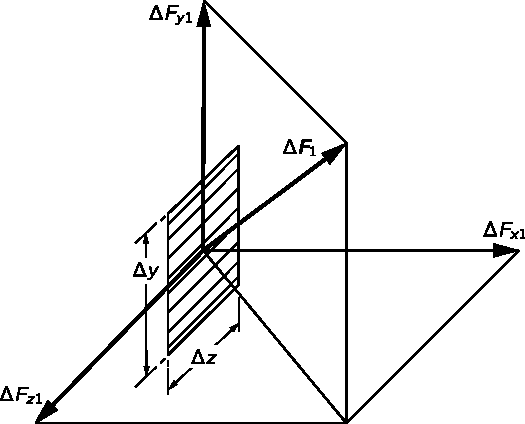
\includegraphics[width=0.8\linewidth]{fyz_fig0879.pdf}
      \caption{\(\Delta F_1\) působící na plošný element \(\Delta y\Delta z\) kolmý na osu \(x\) se
              rozkládá na tři složky \(\Delta F_{x1}\), \(\Delta F_{y1}\) a \(\Delta F_{z1}\)
              (\cite[s.~584]{Feynman02})}
      \label{fyz:fig0879}
    \end{figure}

    Jeden druh napětí už známe, a to statický tlak v kapalině. V tom případě je síla kolmá na
    povrchový element a je rovna tlaku vynásobenému povrchem. Pro pevné látky (jakož i pro
    pohybující se viskózní kapaliny) nemusí být síla kolmá na povrch, působí tu kromě tlaků
    (kladných nebo záporných) i \textbf{smykové síly}. (Smykovou silou rozumíme \emph{tangenciální}
    složku síly působící na povrch.) Všechny tři složky síly je třeba vzít v úvahu. Všimněme si, že
    bude-li mít náš řez rovinou jinou orientaci, budou síly jiné. K úplnému popisu vnitřního napětí
    potřebujeme tenzor.
    
    \emph{Tenzor napětí} definujeme takovýmto způsobem: Představme si nejdříve řez kolmý na osu
    \(x\) a rozložme sílu \(Δ\vec{F_1}\) působící v řezu na složky \(ΔF_{x1}\), \(ΔF_{y1}\),
    \(ΔF_{z1}\){ (obr. \ref{fyz:fig0879}). Podíl těchto sil a plošky \(\Delta y\Delta z\) označujeme
    \(S_{xx}\), \(S_{yx}\) a \(S_{zx}\). Například
    \begin{equation*}
      S_{yx}=\frac{\Delta F_{y1}}{\Delta y\,\Delta z}.
    \end{equation*}
    První index \(y\) se vztahuje ke směru silové složky a druhý index \(x\) ke směru, který má
    kolmice na plochu. Chceme-li, můžeme psát plochu \(\Delta y\Delta z\) jako \(\Delta a_x\), čímž
    myslíme plošný element kolmý na \(x\). Pak
    \begin{equation*}
      S_{yx}=\frac{\Delta F_{y1}}{\Delta a_x}.
    \end{equation*}

    \begin{figure}[ht!] %\ref{fyz:fig0880}
      \centering
      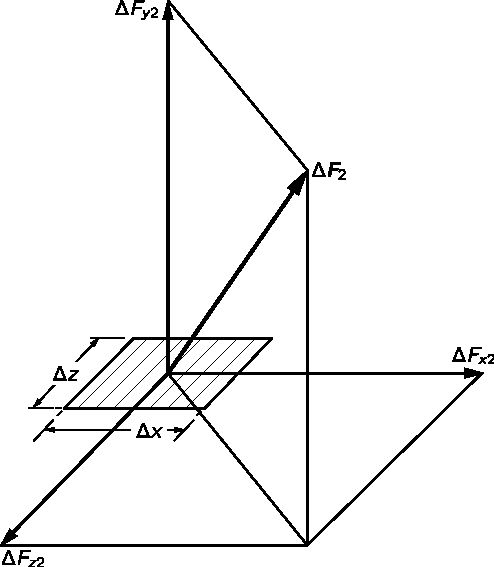
\includegraphics[width=0.8\linewidth]{fyz_fig0880.pdf}
      \caption{Síla působící na plošný element kolmý na \(y\) se rozkládá na tři navzájem kolmé
               složky (\cite[s.~584]{Feynman02})}
      \label{fyz:fig0880}
    \end{figure}

    Dále si představíme řez kolmý na osu \(y\). Na malou plošku \(\Delta x \Delta z\) působí síla
    \(Δ\vec{F_2}\). Opět rozložíme tuto sílu na tři složky tak, jak je to na obr. \ref{fyz:fig0880}.
    Z a definujeme tři složky napětí \(S_{xy}\), \(S_{yy}\), \(S_{zy}\) jako sílu působící na
    jednotkovou plochu ve třech směrech. Nakonec provedeme řez kolmo na \(z\) a definujeme tři
    složky \(S_{xz}\), \(S_{yz}\) a \(S_{zz}\). Máme tedy devět čísel:
    \begin{equation}\label{fyz:eq951}
      S_{ij}=
        \begin{bmatrix}
          S_{xx} & S_{xy} & S_{xz}  \\
          S_{yx} & S_{yy} & S_{yz}  \\
          S_{zx} & S_{zy} & S_{zz}  \\
        \end{bmatrix}.
    \end{equation}

    Nyní chceme ukázat, že těchto devět čísel stačí k úplnému popisu stavu vnitřního napětí a že
    \(S_{ij}\) je skutečně tenzorem. Předpokládejme, že chceme najít sílu působící na povrch pod
    nějakým libovolným úhlem. Můžeme ji určit z \(S_{ij}\)? Ano, můžeme, a to takovýmto způsobem:
    představme si malý, pevný hranol, jehož jedna stěna \(N\) je šikmá a ostatní dvě jsou rovnoběžné
    se souřadnicovými osami. Je-li stěna \(N\) rovnoběžná s osou \(z\), máme trojhranný útvar
    znázorněný na obr. \ref{fyz:fig0881}. (Je to trochu speciální případ, ale dostatečně ilustruje
    obecnou metodu.) Síly napětí působící na hranolek na obr. \ref{fyz:fig0881} jsou v rovnováze
    (přinejmenším v limitě nekonečně malých rozměrů), proto výsledná síla musí být rovna nule. Síly
    působící na stěny rovnoběžné se souřadnicovými osami zjistíme přímo z \(S_{ij}\). Jejich
    vektorový součet musí být roven síle působící na stěnu \(N\) takže tuto sílu umíme určit pomocí
    \(S_{ij}\).

    \begin{figure}[ht!] %\ref{fyz:fig0881}
      \centering
      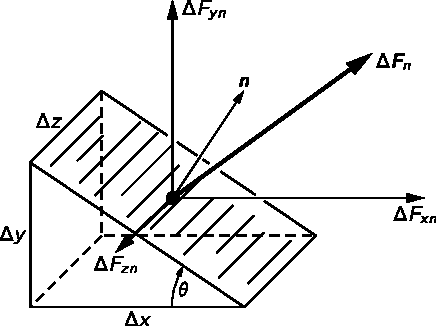
\includegraphics[width=0.8\linewidth]{fyz_fig0881.pdf}
      \caption{Síla\(\Delta F_n\) působící na plochu \(N\) (s jednotkovým vektorem \(\vec{n}\)) se
               rozkládá na tři složky (\cite[s.~585]{Feynman02})}
      \label{fyz:fig0881}
    \end{figure}

    Za našeho předpokladu, že \emph{plošné} síly působící na malý objem jsou v rovnováze,
    zanedbáváme všechny jiné \emph{objemové} síly, které by mohly být přítomny, například gravitaci
    nebo pseudosíly v případě, že naše souřadnicová soustava není inerciální soustavou. Všimněme si
    však, že takové objemové síly budou úměrné objemu hranolku, a tedy úměrné \(ΔxΔyΔz\), zatímco
    plošné síly jsou úměrné ploškám \(ΔxΔy\), \(ΔyΔz\) atd. Proto zvolíme-li si hranolek dostatečně
    malých rozměrů, budou objemové síly vždy zanedbatelné ve srovnání s plošnými silami.
    
    Nyní sečteme všechny síly působící na náš hranolek. Nejdříve vezměme složku \(x\), která je
    sumou pěti částí - po jedné z každé stěny. Je-li však \(Δz\) dostatečně malé, budou síly
    působící na trojúhelníkové stěny (kolmé na osu \(z\)) stejně velké a opačné, můžeme na ně tedy
    zapomenout. Složka \(x\) síly působící na spodní obdélník je
    \begin{equation*}
      \Delta F_{x2}=S_{xy}\,\Delta x\,\Delta z.
    \end{equation*}
    a \(x\)-ová složka síly působící na svislý obdélník je
    \begin{equation*}
      \Delta F_{x1}=S_{xx}\,\Delta y\,\Delta z.
    \end{equation*}
    Součet těchto dvou sil musí být roven \(x\)-ové složce síly působící na plochu \(N\) a směřující
    \emph{ven}. Nechť \(\vec{n}\) je jednotkový vektor kolmý na plochu \(N\) a \(\vec{F_n}\) nechť
    je síla působící na \(N\). Pak máme
    \begin{equation*}
      \Delta F_{xn}=S_{xx}\,\Delta y\,\Delta z+S_{xy}\,\Delta x\,\Delta z.
    \end{equation*}
    Složka \(S_{xn}\) napětí působícího na tuto plochu je rovna \(\Delta F_{xn}\) dělenému velikostí
    plochy \(\Delta z\sqrt{\Delta x^2+\Delta y^2}\), tj.
    \begin{equation*}
      S_{xn}=S_{xx}\,\frac{\Delta y}{\sqrt{\Delta x^2+\Delta y^2}}+
      S_{xy}\,\frac{\Delta x}{\sqrt{\Delta x^2+\Delta y^2}}.
    \end{equation*}
    Výraz \(\Delta x/\sqrt{\Delta x^2+\Delta y^2}\) je však kosinem úhlu \(\theta\) jenž svírají
    vektor \(\vec{n}\) a osa \(y\), jak to vidíme na obr. \ref{fyz:fig0881} - lze jej proto psát jako
    složkuy vektoru \(\vec{n}\), tj. jako \(n_y\). Podobně pro \(\Delta y/\sqrt{\Delta x^2+\Delta
    y^2}\) platí \(\sin\theta=n_x\). Můžeme psát
    \begin{equation*}
      S_{xn}=S_{xx}n_x+S_{xy}n_y.
    \end{equation*}
    Zobecníme-li to nyní na libovolný elementární povrch, dostaneme
    \begin{equation*}
      S_{xn}=S_{xx}n_x+S_{xy}n_y+S_{xz}n_z
    \end{equation*}
    nebo obecně
    \begin{equation}\label{fyz:eq952}
      S_{in}=\sum_jS_{ij}n_j.
    \end{equation} 
    Je tedy možné vyjádřit sílu působící na libovolnou elementární plochu pomocí koeficientů
    \(S_{ij}\), které tak úplně popisují vnitřní napětí v látce.

    \begin{figure}[ht!] %\ref{fyz:fig0882}
      \centering
      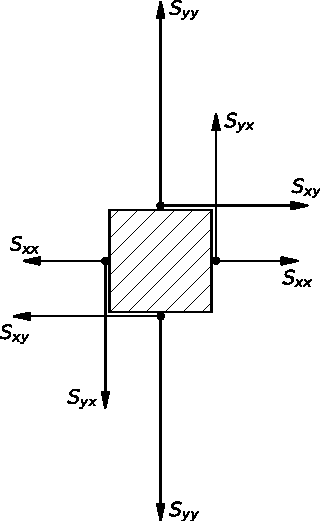
\includegraphics[width=0.7\linewidth]{fyz_fig0882.pdf}
      \caption{Složky sil \(x\) a \(y\) působících na čtyři stěny malé jednotkové krychle
               (\cite[s.~586]{Feynman02})}
      \label{fyz:fig0882}
    \end{figure}

    Rovnice \eqref{fyz:eq952} nám říká, že tenzor \(S_{ij}\) dává do vztahu sílu \(\vec{S_n}\) a
    jednotkový vektor \(\vec{n}\) právě tak, jako \(\alpha_{ij}\), dává do vztahu \(\vec{P}\) a
    \(\vec{E}\). Jelikož \(\vec{n}\) a \(\vec{S_n}\) jsou vektory, musí se složky \(S_{ij}\)
    transformovat při změně souřadnic jako tenzor. \(S_{ij}\) je tedy skutečně tenzorem.

    Jelikož \(S_{ij}\) je symetrickým tenzorem, může být popsán elipsoidem se třemi hlavními osami.
    Pro plochy kolmé na tyto osy jsou napětí obzvlášť jednoduchá - odpovídají tlaku nebo tahu
    kolmému na danou plochu. Podél těchto ploch nepůsobí žádné smykové síly. Pro \emph{libovolné}
    napětí můžeme vždy zvolit naše osy tak, aby byla smyková složka síly rovna nule. Je-li
    elipsoidem koule, působí v \emph{libovolném} směru jen kolmé složky. To odpovídá hydrostatickému
    tlaku (kladnému nebo zápornému). Pro hydrostatický tlak je tedy tenzor diagonální a všechny tři
    složky jsou navzájem rovny. Ve skutečnosti jsou rovny právě tlaku \(p\). Můžeme psát
    \begin{equation}\label{fyz:eq953}
      S_{ij}=p\delta_{ij}.
    \end{equation}

    Tenzor napětí, jakož i jeho elipsoid, se budou obecně měnit v dané látce od bodu k bodu.
    Chceme-li popsat daný kus látky, musíme udat hodnotu každé složky \(S_{ij}\) jako funkci polohy.
    Tenzor napětí je tedy \textbf{polem}. Poznali jsme už skalární pole, jako například teplotu
    \(T(x,y,z)\), v nichž je každému bodu v prostoru přiděleno jedno číslo, a vektorová pole jako
    \(\vec{E(x,y,z)}\), v nichž se každému bodu přiřazuje trojice čísel. Nyní máme tenzorové pole,
    kde je každému bodu prostoru přiřazeno devět čísel, nebo vlastně šest, protože \(S_{ij}\), je
    symetrický tenzor. Pro úplný popis vnitřních sil působících v libovolně deformované látce
    potřebujeme šest funkcí proměnných \(x, y, z\).
 
  \section{Tenzory vyššího řádu}\label{fyz:IIchapXXXIsecVII}
    
    Tenzor napětí \(S_{ij}\) popisuje \emph{vnitřní síly} v látce. Je-li látka elastická, je výhodné
    popisovat vnitřní \textbf{deformace} pomocí jiného tenzoru \(T_{ij}\), která se nazývá tenzor
    \emph{deformace}. Pro jednoduchý objekt, jako je například kovová tyč, umíme určit změnu délky
    \(ΔL\) podle \emph{Hookova zákona}, který říká, že prodloužení je přibližně úměrné síle:
    \begin{equation*}
      \Delta L=\gamma F.
    \end{equation*}
    
    Pro libovolné deformace pružného tuhého tělesa je vztah mezi deformací \(T_{ij}\) a napětím
    \(S_{ij}\) určen systémem lineárních rovnic 
    \begin{equation}\label{fyz:eq954}
      T_{ij}=\sum_{k,l}\gamma_{ijkl}S_{kl}.
    \end{equation}
    Také víme, že potenciální energie pružiny (nebo tyče) je rovna
    \begin{equation*}
      \dfrac{1}{2}F\,\Delta L=\dfrac{1}{2}\gamma F^2.
    \end{equation*}    
    Obecný výraz pro hustotu elastické energie pevného tělesa je
    \begin{equation}\label{fyz:eq955}
      U_{\text{elastic}}=\sum_{ijkl}\dfrac{1}{2}\gamma_{ijkl}S_{ij}S_{kl}.
    \end{equation}
    
    Úplný popis elastických vlastností krystalu je určen koeficienty \(\gamma_{ijkl}\). Tímto
    představujeme novou „obludu“ - \textbf{tenzor čtvrtého řádu}. Jelikož každý index může nabývat
    libovolnou ze tří hodnot \(x\), \(y\) nebo \(z\), dostáváme dohromady \(3^4 = 81\) koeficientů.
    Jenže ve skutečnosti je to jen 21 různých čísel. Zaprvé, jelikož tenzor \(S_{ij}\) je
    symetrický, obsahuje jen šest různých hodnot a v rovnici \eqref{fyz:eq955} potřebujeme jen 36
    \emph{různých} koeficientů. Zároveň však můžeme zaměnit \(S_{IJ}\) za \(S_{kl}\), aniž bychom
    změnili energii, proto \(\gamma_{ijkl}\) musí být symetrický při záměně \(ij\) za \(KL\). Tím se
    snižuje počet různých koeficientů na 21. Proto K popisu elastických vlastností krystalu s
    nejnižší možnou symetrií je třeba 21 elastických konstant! Tento počet je, samozřejmě, nižší pro
    krystaly s vyšší symetrií. Například krychlový krystal má jen tři pružné konstanty a izotropní
    látka má jen dvě.
    
    O správnosti předcházejícího tvrzení se můžeme přesvědčit. Jak mohou být složky tenzoru
    \(\gamma_{ijkl}\) nezávislé na směru os tak, jak to vyžadujeme pro izotropní látky? Odpověď je
    následující. Mohou být nezávislé \emph{jen} tehdy, když je lze vyjádřit pomocí tenzoru
    \(\delta_{ij}\). Existují dva možné výrazy \(\delta_{ij}\delta_{kl}\) a
    \(\delta_{ik}\delta_{jl}+\delta_{il}\delta_{jk}\) které mají požadovanou symetrii, proto
    \(\gamma_{ijkl}\) musí být jejich lineární kombinací. Proto pro izotropní látky platí
    \begin{equation*}
      \gamma_{ijkl}=a(\delta_{ij}\delta_{kl})+b(\delta_{ik}\delta_{jl}+\delta_{il}\delta_{jk}),
    \end{equation*}
    a potřebujeme dvě konstanty \(a\) a \(b\) k popisu elastických vlastností látky. Důkaz, že
    krychlový krystal potřebuje tři konstanty, přeskočíme.
    
    Jako poslední příklad, tentokrát na tenzor třetího řádu, uvádíme piezoelektrický efekt.
    Působením napětí se v krystalu vytváří elektrické pole úměrné napětí. Obecný zákon má tvar
    \begin{equation*}
      E_i=\sum_{j,k}P_{ijk}S_{jk},
    \end{equation*}
    kde \(E_i\) je elektrické pole a \(P_{ijk}\) jsou piezoelektrické koeficienty nebo
    piezoelektrický tenzor. Uměli bychom dokázat, že má-li krystal střed inverze (invariance při
    záměně \(x,y,z\to-x,-y,-z\) všechny piezoelektrické koeficienty jsou rovny nule?

  \section{Čtyřtenzor elektromagnetické energie a hybnosti}\label{fyz:IIchapXXXIsecVIII} 
    Všechny tenzory, které jsme v této kapitole dosud probírali, se vztahují k trojrozměrnému
    prostoru. Jsou definovány jako veličiny, které mají určité transformační vlastnosti při
    trojrozměrných rotacích. V kapitole \ref{fyz:IIchapXXVI} jsme měli možnost pracovat s tenzorem
    ve \emph{čtyřrozměrném relativistickém časoprostoru}, a to s tenzorem elektromagnetického pole
    \(F_{\mu\nu}\). Složky takového čtyřtenzoru se při Lorentzově transformaci souřadnic
    transformují určitým způsobem, který jsme odvodili. (Ačkoli jsme to tak nedělali, mohli jsme
    Lorentzovy transformace považovat za „rotace“ ve čtyřrozměrném „prostoru“, který se nazývá
    \emph{Minkowského prostor}. Pak by i analogie s tím, co nyní děláme, byla jasnější.)
    
    Jako náš poslední příklad zmíníme ještě jeden čtyřrozměrný tenzor z teorie relativity. Když jsme
    hovořili o tenzoru napětí, definovali jsme \(S_{ij}\) jako složky sil působících na jednotlivé
    plochy. Ale síla je rovna časové změně hybnosti. Proto místo výroku „\(S_{xy}\) je složkou \(x\)
    síly působící na jednotkovou plochu kolmou na \(y\)“ bychom stejně správně mohli říci
    „\(S_{xy}\) je rychlost změny toku složky \(x\) hybnosti jednotkovou plochou kolmou na \(y\).
    Jinými slovy, každá složka \(S_{ij}\) představuje i hustotu toku \(i\)-té složky hybnosti
    jednotkovou plochou kolmou na směr \(j\). Tyto čistě prostorové složky jsou však součástí
    „většího“ tenzoru \(S_{\mu\nu}\) ve čtyřech rozměrech (\(\mu\) a \(v= t, x,y,z\), který obsahuje
    navíc složky typu \(S_{xx}\), \(S_{xy}\), a \(S_{xz}\) atd. Nyní se pokusíme najít fyzikální
    význam těchto dodatečných složek.
    
    Víme, že prostorové složky představují hustotu toku hybnosti. Klíč k interpretaci časové složky
    nám poskytne jiný druh „toku“ - tok elektrického náboje. Rychlosti toku \emph{skalární}
    veličiny, náboje (jednotkovou plochou kolmou na tok), přiřazujeme prostorový vektor - vektor
    proudové hustoty \(\vec{j}\). Viděli jsme, že časová složka tohoto vektoru toku představuje
    hustotu toho, co teče. Například \(\vec{j}\) můžeme kombinovat s hustotou náboje \(\varrho\) a
    dostaneme čtyřvektor \(j_\mu=(\varrho,\vec{j})\) tj. index \(\mu\) v \(i_\mu\) nabývá hodnoty
    \(t\), \(x\), \(y\), \(z\), což postupně označuje hustotu, hustotu toku ve směru \(x\), hustotu
    toku ve směru \(y\) hustotu toku ve směru \(z\) skalárního náboje.
    
    Nyní, v analogii s naším tvrzením o časové složce toku skalární veličiny, bychom mohli očekávat,
    že vedle \(S_{xx}\), \(S_{xy}\), a \(S_{xz}\), které popisují tok \(x\)-ové složky hybnosti,
    existuje i časová složky \(S_{xt}\), která představuje hustotu toho, co teče, tj. \(S_{xt}\) by
    měla být hustotou \(x\)-ové složky hybnosti. Náš tenzor tak můžeme horizontálně rozšířit o
    složku \(t\). Dostaneme:
    \begin{itemize}[noitemsep]
      \item \(S_{xt}\ldots\) hustota \(x\)-ové složky hybnosti,
      \item \(S_{xx}\ldots\) hustota toku \(x\)-ové složky hybnosti ve směru \(x\),
      \item \(S_{xy}\ldots\) hustota toku \(x\)-ové složky hybnosti ve směru \(y\),
      \item \(S_{xz}\ldots\) hustota toku \(x\)-ové složky hybnosti ve směru \(z\).
    \end{itemize}
    Podobně pro \(y\)-ovou složku hybnosti máme tři složky hustoty toku \(S_{yx}\), \(S_{yy}\),
    \(S_{yz}\), k nimž přidáme čtvrtou složku
    
    \begin{center}
      \(S_{yt}\) = hustota \(y\)-ové složky hybnosti.
    \end{center}

    A samozřejmě, k \(S_{zz}\) bychom měli přidat
    \begin{center}
      \(S_{zt}\) = hustota \(z\)-ové složky hybnosti.
    \end{center}
    
    Ve čtyřech rozměrech existuje i složka \(t\) hybnosti, a to je, jak víme, energie. Proto by
    tenzor \(S_{ij}\) měl být rozšířen i vertikálně o složky \(S_{tx}\), \(S_{ty}\), a \(S_{tz}\)
    kde
    \begin{itemize}[noitemsep]
      \item \(S_{tx}\ldots\) hustota toku energie ve směru \(x\),
      \item \(S_{ty}\ldots\) hustota toku energie ve směru \(y\),
      \item \(S_{tz}\ldots\) hustota toku energie ve směru \(z\).
    \end{itemize}
    tj. \(S_{tx}\) je tok energie jednotkovou plochou kolmou k ose \(x\) na jednotku času atd.
    Nakonec, abychom zkompletovali náš tenzor, potřebujeme \(S_{tt}\) a to by měla být
    \textbf{hustota energie}. Náš trojrozměrný tenzor napětí \(S_{ij}\) jsme tak rozšířili na
    \textbf{čtyřrozměrný tenzor energie a hybnosti} \(S_{\mu\nu}\). Index \(\mu\) může nabývat čtyř
    hodnot \(t\), \(x\), \(y\), \(z\), které postupně označují hustotu, hustotu toku ve směru \(x\)
    hustotu toku ve směru \(y\) a hustotu toku ve směru \(z\). Podobně \(\nu\) nabývá čtyř hodnot
    \(t\), \(x\), \(y\), \(z\), které označují to, \emph{co} teče: energii, hybnost ve směru \(x\)
    hybnost ve směru \(y\) a hybnost ve směru \(z\).
    
    Jako příklad budeme tento tenzor uvažovat ne v látce, ale v nějaké oblasti volného prostoru, kde
    působí elektromagnetické pole. Víme, že hustota toku energie je určena \emph{Poyntingovým
    vektorem} \(\vec{S}=\epsilon_0c^2\vec{E}\times\vec{B}\). Z relativistického hlediska jsou složky
    \(x\), \(y\), \(z\) vektoru \(\vec{S}\) složkami \(S_{tx}\), \(S_{ty}\), a \(S_{tz}\) našeho
    čtyřrozměrného tenzoru energie a hybnosti. Symetrie tenzoru \(S_{ij}\) platí stejně i pro časové
    složky, proto je čtyřrozměrný tenzor \(S_{\mu\nu}\) symetrický
    \begin{equation}\label{fyz:eq956}
      S_{\mu\nu}=S_{\nu\mu}.
    \end{equation}
    Jinými slovy, složky \(S_{xt}\), \(S_{yt}\), \(S_{zt}\), které představují hustoty složek \(x\),
    \(y\) a \(z\) hybnosti, jsou zároveň složkami \(x\), \(y\) a \(z\) Poyntingova vektoru
    \(\vec{S}\), který představuje hustotu toku energie, jak jsme už ukázali v jedné z
    předcházejících kapitol.
    
    Zbývající složky elektromagnetického tenzoru energie a hybnosti \(S_{\mu\nu}\) lze také vyjádřit
    pomocí elektrického a magnetického pole \(\vec{E}\) a \(\vec{B}\). Musíme tedy připustit
    existenci napětí nebo, aby to neznělo tak záhadně, existenci toku hybnosti v elektromagnetickém
    poli. Mluvili jsme o tom v kapitole \ref{fyz:IIchapXXVII} v souvislosti s rovnicí
    \eqref{fyz:eq957}, ale tehdy jsme nešli do detailů.
    
    Chceme-li si vyzkoušet svou zručnost v zacházení s tenzory ve čtyřech rozměrech, je dobré
    vědět, jak \(S_{\mu\nu}\) vyjádřit pomocí polí:
    \begin{equation*}
      S_{\mu\nu}=-\varepsilon_0\biggl(
      \sum_\alpha F_{\mu\alpha}F_{\nu\alpha}-\dfrac{1}{4}\delta_{\mu\nu}
      \sum_{\alpha,\beta}F_{\beta\alpha}F_{\beta\alpha}
      \biggr),
    \end{equation*}
    kde sčítání přes \(\alpha\), \(\beta\) znamená sčítání přes \(t\), \(x\), \(y\), \(z\), ale (jak
    to bývá zvykem v teorii relativity) sumační znak \(\sum\) a symbol \(\delta\) mají speciální
    význam. Při sumaci se členy s \(x\), \(y\), \(z\) odčítají a \(δ_{tt}=+1\), zatímco \(δ_{xx} =
    δ_{yy} = δ_{zz}= −1\) a \(δ_{μ\nu}=0\) pro \(μ≠ν\) (\(c=1\)). Uměli bychom ověřit, že toto
    vyjádření vede k hustotě energie \(S_{tt}=(\varepsilon_0/2)\,(E^2+B^2)\) a k Poyntingovu vektoru
    \(\varepsilon_0\vec{E}\times\vec{B}\)? Uměli bychom ukázat, že v elektrostatickém poli, kde
    \(\vec{B}= 0\), mají hlavní osy napětí směr elektrického pole a že ve směru pole vzniká napětí
    \((\varepsilon_0/2)E^2\), zatímco ve směru kolmém na pole vzniká stejně velký \emph{tlak}?